\documentclass{article}
\usepackage{amsmath, amsfonts, graphicx, fullpage, leftidx}
\begin{document}
\section{Pole/end-effector sub system}
Consider a massless pole with a sphere attached to one end, with sphere mass being $m_s$. The other end of the pole (point $A$) is attached to the end-effector with mass $m_e$ at point $A$. The state of the system is the velocity of the end-effector point A $(\dot{x}_A, \dot{y}_A, \dot{z}_A)$, the delta position between the sphere and the end-effector in the horizontal plane $x_{AB} = x_B - x_A, y_{AB} = y_B-y_A$, together with its time derivative $\dot{x}_{AB}, \dot{y}_{AB}$.

\begin{figure}
	\centering
	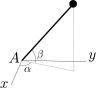
\includegraphics[width=0.5\textwidth]{pole.pdf}
\end{figure}

The position of the mass is
\begin{align}
	\begin{bmatrix}
		x_A + x_{AB}\\
		y_A + y_{AB}\\
		z_A + \sqrt{l^2 - x_{AB}^2 - y_{AB}^2}
	\end{bmatrix}
\end{align}
The velocity of the mass is
\begin{align}
	\begin{bmatrix}
		\dot{x}_A + \dot{x}_{AB}\\
		\dot{y}_A + \dot{y}_{AB}\\
		\dot{z}_A - \frac{x_{AB}\dot{x}_{AB} + y_{AB}\dot{y}_{AB}}{\sqrt{l^2-x_{AB}^2 - y_{AB}^2}}
	\end{bmatrix}
\end{align}
The total kinetic energy of the system is
\begin{multline}
	T = 0.5 m_e (\dot{x}_A^2 + \dot{y}_A^2 +\dot{z}_A^2) + 0.5 m_s(\dot{x}_A^2 + \dot{y}_A^2 + \dot{z}_A^2 + \dot{x}_{AB}^2 + \dot{y}_{AB}^2 + \frac{(x_{AB}^2\dot{x}_{AB}^2 + y_{AB}^2\dot{y}_{AB}^2 + 2x_{AB}y_{AB}\dot{x}_{AB}\dot{y}_{AB})}{l^2-x_{AB}^2-y_{AB}^2}\\
	+ 2\dot{x}_A\dot{x}_{AB} + 2\dot{y}_A\dot{y}_{AB} - \frac{2\dot{z}_A(x_{AB}\dot{x}_{AB}+y_{AB}\dot{y}_{AB})}{\sqrt{l^2-x_{AB}^2-y_{AB}^2}})
\end{multline}
The total potential energy is
\begin{align}
	V = m_egz_A + m_sg(z_A + \sqrt{l^2-x_{AB}^2-y_{AB}^2})
\end{align}
Using Lagrangian $L = T-V$ and $\frac{d}{dt}\frac{\partial L}{\partial \dot{q}}-\frac{\partial L}{\partial q} = Bu$, we have
\begin{align}
	(m_e + m_s)\ddot{x}_A + m_s\ddot{x}_{AB} = f_x\\
	(m_e + m_s)\ddot{y}_A + m_s\ddot{y}_{AB} = f_y
\end{align}
\begin{multline}
	(m_e + m_s)(\ddot{z}_A+g) - m_s\left(\dot{x}_{AB}^2\frac{l^2 - y_{AB}^2}{z_{AB}^3} + \frac{x_{AB}}{z_{AB}}\ddot{x}_{AB} + \dot{y}_{AB}^2\frac{l^2-x_{AB}^2}{z_{AB}^3} + \frac{y_{AB}}{z_{AB}}\ddot{y}_{AB} - 2 \frac{x_{AB}y_{AB}\dot{x}_{AB}\dot{y}_{AB}}{z_{AB}^3}\right) = f_z
\end{multline}
\begin{multline}
	m_s(\ddot{x}_A + \ddot{x}_{AB}) - m_sx_{AB}(g+\ddot{z}_A)/z_{AB} + m_s(x_{AB}^2\ddot{x}_{AB}+x_{AB}\dot{x}_{AB}^2+x_{AB}y_{AB}\ddot{y}_{AB}+x_{AB}\dot{y}_{AB}^2)/z_{AB}^2\\
	+ m_s(x_{AB}^3\dot{x}_{AB}^2 + 2x_{AB}^2y_{AB}\dot{x}_{AB}\dot{y}_{AB} + x_{AB}y_{AB}^2\dot{y}_{AB}^2)/z_{AB}^4=0
\end{multline}
\begin{multline}
	m_s(\ddot{y}_A + \ddot{y}_{AB}) - m_sy_{AB}(g+\ddot{z}_A)/z_{AB} + m_s(y_{AB}^2\ddot{y}_{AB}+y_{AB}\dot{y}_{AB}^2+y_{AB}x_{AB}\ddot{x}_{AB}+y_{AB}\dot{x}_{AB}^2)/z_{AB}^2\\
	+ m_s(y_{AB}^3\dot{y}_{AB}^2 + 2y_{AB}^2x_{AB}\dot{y}_{AB}\dot{x}_{AB} + y_{AB}x_{AB}^2\dot{x}_{AB}^2)/z_{AB}^4=0
\end{multline}

In the matrix form, we have
\begin{align}
	M	\begin{bmatrix}\ddot{x}_A\\\ddot{y}_A\\\ddot{z}_A\\\ddot{x}_{AB}\\\ddot{y}_{AB}\end{bmatrix} + C = \begin{bmatrix}f_x\\f_y\\f_z\\0\\0\end{bmatrix}\label{eq:pole_ee_manipulator_eq}
\end{align}
where
\begin{align}
	M = 
	\begin{bmatrix}
		m_e + m_s & 0 & 0 & m_s & 0\\
		0 & m_e + m_s & 0 & 0 & m_s\\
		0 & 0 & m_e + m_s & -m_s\frac{x_{AB}}{z_{AB}} & -m_s\frac{y_{AB}}{z_{AB}}\\
		m_s& 0 & -m_s\frac{x_{AB}}{z_{AB}} & m_s + m_s\frac{x_{AB}^2}{z_{AB}^2} & m_s\frac{x_{AB}y_{AB}}{z_{AB}^2}\\
		0 & m_s & -m_s\frac{y_{AB}}{z_{AB}} &m_s\frac{x_{AB}y_{AB}}{z_{AB}^2} & m_s + m_s\frac{y_{AB}^2}{z_{AB}^2}
	\end{bmatrix}\\
	C = \begin{bmatrix}
		0\\
		0\\
		(m_e + m_s)g - m_s\left(\dot{x}_{AB}^2\frac{l^2-y_{AB}^2}{z_{AB}^3} + \dot{y}_{AB}^2\frac{l^2-x_{AB}^2}{z_{AB}^3} - 2\frac{x_{AB}y_{AB}\dot{x}_{AB}\dot{y}_{AB}}{z_{AB}^3}\right)\\
		-m_sg\frac{x_{AB}}{z_{AB}}+m_sx_{AB}\left(\frac{\dot{x}_{AB}^2 + \dot{y}_{AB}^2}{z_{AB}^2}+\frac{(x_{AB}\dot{x}_{AB} + y_{AB}\dot{y}_{AB})^2}{z_{AB}^4}\right)\\
		-m_sg\frac{y_{AB}}{z_{AB}}+m_sy_{AB}\left(\frac{\dot{x}_{AB}^2 + \dot{y}_{AB}^2}{z_{AB}^2}+\frac{(x_{AB}\dot{x}_{AB} + y_{AB}\dot{y}_{AB})^2}{z_{AB}^4}\right)
	\end{bmatrix}
\end{align}

\section{Whole system}
Assuming that we construct a controller, that given the current state of the pole/end-effector system, this controller computes the force $f_x, f_y, f_z$ applied from the robot to the end-effector, now we want to compute the robot joint torque $\tau$ to apply that force.

We first apply the force $f_x, f_y, f_z$ computed from the controller as input to the pole/end-effector system, from the dynamics equation \eqref{eq:pole_ee_manipulator_eq} we can compute the acceleration of the end effector $\ddot{x}_A, \ddot{y}_A, \ddot{z}_A$, together with the acceleration of the pole $\ddot{x}_B, \ddot{y}_B, \ddot{z}_B$ (where we use both $\ddot{x}_A, \ddot{y}_A, \ddot{z}_A$ and $\ddot{x}_{AB}, \ddot{y}_{AB}, \ddot{z}_{AB}$). We know that for the pole to achieve this acceleration, the end-effector has to apply a force
\begin{align}
	f_B = m_s\begin{bmatrix}\ddot{x}_B \\ \ddot{y}_B \\ \ddot{z}_B + g\end{bmatrix}
\end{align}
onto the pole, applied at where the pole makes contact with the end effector. Based on Newton's third law, there is an equal and opposite force $-f_B$ applied on the end-effector at the contact point $P$ between the end-effector and the pole. Hence our goal is to compute the joint torque of the robot arm, such that the end-effector can achieve the desired acceleration $\ddot{x}_A, \ddot{y}_A, \ddot{z}_A$ under the external force $-f_B$.

We can write the manipulator equation for the IIWA arm (together with the end-effector welded to the wrist joint)
\begin{align}
	M_{iiwa}\ddot{q}_{iiwa} + C = g(q_{iiwa}) + \tau - \left(\leftidx{^W}{J}^P\right)^Tf_B\label{eq:iiwa_eom}
\end{align}
where $\leftidx{^W}{J}^P$ is the Jacobian of the contact point $P$ written in the world frame.
And we also have the constraints on the end-effector acceleration
\begin{align}
	\leftidx{^W}{J}^E\ddot{q}_{iiwa} + \leftidx{^W}{\dot{J}}^E\dot{q}_{iiwa} = \leftidx{^W}{a}^E_{des}\label{eq:iiwa_ee_acceleration}
\end{align}
where $\leftidx{^W}{J}^E$ is the Jacobian of the end-effector written in the world frame. $\leftidx{^W}{a}^E_{des}$ is the desired acceleration of the IIWA end-effector frame $E$ in the world frame $W$. This acceleration includes both the linear acceleraton $\ddot{x}_A, \ddot{y}_A, \ddot{z}_A$, together with the desired angular acceleration. The desired acceleration can be set in two ways
\begin{itemize}
	\item If our goal is to keep the end-effector to be horizontal, then we can compute the desired angular acceleration using a PD law depending on the orientation error.
	\item We can also set the desired end-effector acceleration to be zero. Note that this won't handle any orientation drift. Namely if currently the end-effector angular velocity is non-zero, then the orientation will continue to drift.
\end{itemize}

Combining the equations \eqref{eq:iiwa_eom} and \eqref{eq:iiwa_ee_acceleration} we have unknown variable $\tau\in\mathbb{R}^7$. The problem is under-constrained, we can also impose the cost as $\min \tau^T\tau$ to get a unique (and optimal) $\tau$. If we ignore the joint torque limit, then this ends up being an equality-constrained QP which can be solved very efficiently in the closed form.

\end{document}
